\documentclass[12pt,a4paper]{article} 
\usepackage[a4paper,margin=2cm]{geometry}

\usepackage{cmap}
\usepackage[french]{babel}
\usepackage[T1]{fontenc}
\usepackage[utf8]{inputenc}
\usepackage[kerning=true]{microtype}
\usepackage{lmodern}

\usepackage{amsmath}
\usepackage{amsfonts}
\usepackage{amssymb}
\usepackage{graphicx}

\usepackage{hyperref}

\makeatletter

\title{\vspace{-3ex}\textbf{Rapport:\\ Compilateur Petit Purescript}}
\author{Matthieu Boyer, Antoine Groudiev}
\date{}

\begin{document}
\maketitle

Ce document vise à détailler les différents choix techniques que nous avons pris lors de la réalisation de notre compilateur, et à guider le lecteur dans la compréhension de notre code source.

\section{Exécution}
\begin{itemize}
    \item La commande \texttt{make} créé le compilateur, nommé \texttt{ppurs}, à la racine du projet.
    \item La commande \texttt{make test} créé et exécute le compilateur sur le fichier par défaut \texttt{test.purs}.
    \item La commande \texttt{make testc} créé et exécute le compilateur sur le fichier par défaut \texttt{test.purs}, et lance l'exécution avec \texttt{gcc}.
    \item La commande \texttt{make testd} est similaire à \texttt{make testd} mais active le mode \texttt{dbg}, qui \emph{pretty print} l'AST.
    \item La commande \texttt{make tests1} exécute le compilateur sur les jeux de tests de la partie 1 (respectivement 2 et 3).
    \item La commande \texttt{make clean} supprime les fichiers créés par \texttt{make}
\end{itemize}

Une fois créé, le compilateur peut être exécuté en lançant une commande de la forme:
\begin{center}
    \texttt{./ppurs [options] file.purs}
\end{center}
Les différentes options disponibles sont listées par la commande \texttt{./ppurs --help}, parmi lesquelles les options demandées d'analyse syntaxique ou typage seuls, et un mode de déboggage qui affiche l'AST.

\section{Choix techniques}
Le langage utilisé est OCaml. L'analyse lexicale est faite à l'aide de l'outil \texttt{ocamllex}, et l'analyse syntaxique avec Menhir.

\subsection{Fichiers généralistes}
\texttt{ppurs.ml} est le fichier principal du projet. Il traite les arguments de la ligne de commande, appelle successivement les différents analyseurs, et gère les éventuelles erreurs advenant au cours de la compilation.

Le fichier \texttt{utility.ml} contient des fonctions utilitaires servant notamment à extraire l'addresse ou le type d'une expression, d'un atome, etc.

\subsection{Analyse lexicale}
\texttt{lexer.mll} contient un analyseur lexical traditionnel, dans le sens où il ne gère pas l'indentation significative. 

À la place, est \texttt{indenter.ml} contient un second analyseur lexical. 
Son rôle est de traiter correctement l'indentation significative propre à PureScript, en générant à la volée les tokens factices \texttt{SEMICOLON} (\texttt{;}), \texttt{LBRACK} (\texttt{\{}) et \texttt{RBRACK} (\texttt{\}}) parmi le flux de lexèmes généré par \texttt{lexer.mll}.
La fonction principale de ce fichier, \texttt{traiter\_lexeme}, reproduit le comportement attendu d'un analyseur lexical.
Elle a ainsi sensiblement le même type que \texttt{Lexer.token}, à l'exception du booléen précisant le type (fort ou faible) voulu.

\subsection{Analyse syntaxique}
\texttt{parser.mly} contient l'analyseur syntaxique. Son comportement est standard et suit majoritairement la grammaire PureScript telle que détaillée dans le sujet. Une exception notable est la règle \texttt{tdecl}, qui nous a posé des difficultés à parser. La technique adoptée a été de lire la liste à la main, à l'aide d'une règle \texttt{type\_list} qui implémente manuellement et plus finement la construction \texttt{list} de Menhir. Pour pouvoir localiser précisément les erreurs de typage, les types \texttt{expr}, \texttt{atom}, et \texttt{patarg} sont transformés par le parser en \texttt{loc\_expr}, \texttt{loc\_atom}, et \texttt{loc\_patarg}, qui sont décorés des informations de localisation.

L'arbre de syntaxe abstraite généré par l'analyse syntaxique est défini dans \texttt{ast.ml}, comme les deux autres AST (respectivement après le typage et l'allocation des variables.)

\subsection{Typage}
\texttt{typing.ml} contient l'analyseur sémantique. L'algorithme employé est le suivant : on type une à une les déclarations du fichier, en maintenant dans des tables de hachage, qui contiennent les définitions de fonctions, de types, de classes et d'instances. On vérifie à chaque étape que la liste des définitions à l'intérieur d'une déclaration (\texttt{fdecl}, \texttt{clas}, \texttt{data}, \texttt{instance} dans le type \texttt{decl}) est bien regroupée par nom de fonction, et que celle-ci ne déborde pas de la déclaration. Dans chaque définition (\texttt{defn} dans le type \texttt{decl}), on vérifie récursivement le type de chaque morceau selon la construction de l'arbre de syntaxe. 

A été fait le choix de séparer les différentes erreurs de typage en de nombreuses exceptions, comme le traduit les premières lignes du fichier. Cette séparation est en fait peu utile en pratique pour un compilateur de faible ampleur, mais nous semblait plus propre et plus \emph{scalable}.

\subsection{Production de code}
Le fichier \texttt{compile.ml} est séparé en deux parties: l'allocation sur la pile, et la production du code assembleur.  

\subsubsection{Allocation}
Le schéma de compilation et particulièrement d'allocation est similaire à celui décrit dans le sujet. Les valeurs de retour des fonctions sont cependant stockées sur la pile, et non pas dans le registre \texttt{\%rax}.

C'est également à cette étape que les éventuels \emph{pattern matching} faisant intervenir plusieurs déclarations de fonctions sont convertis en un \texttt{case}, dans la fonction \texttt{alloc}. (Ceci aurait dû plus logiquement être fait pendant le typage.)

\subsubsection{Compilation}
Au fichier \texttt{x86\_64.ml} a été rajouté deux constructions: l'instruction \texttt{enter} de \texttt{x86-64}, pour une gestion de la pile plus aisée, et une instruction \texttt{comment}, permettant d'insérer des commentaires dans le code, très utile pour le déboggage. 

Certaines fonctions ont naturellement été écrites directement en assembleur. C'est le cas des fonctions d'affichage d'entiers, de booléens, de division et modulo, de concaténation de chaînes, mais aussi des fonctions prédéfinies de PureScript, telles \texttt{log}, \texttt{not} ou \texttt{pure}. À noter que ces fonctions ne sont ajoutées au code que si potentiellement utilisées.

\subsection{\emph{Pretty printer}}
Le fichier \texttt{pretty.ml} contient un \emph{pretty printer} pour les arbres après le typage et après l'allocation. Il affiche, en couleur, la hierarchie des constructions et les "adresses" des variables et autres données allouées, et s'est avéré très utile lors des nombreuses phases de déboggage. Il peut notamment être affiché en activant l'option \texttt{\textendash \textendash dbg}.

\begin{figure}[!h]
    \center
    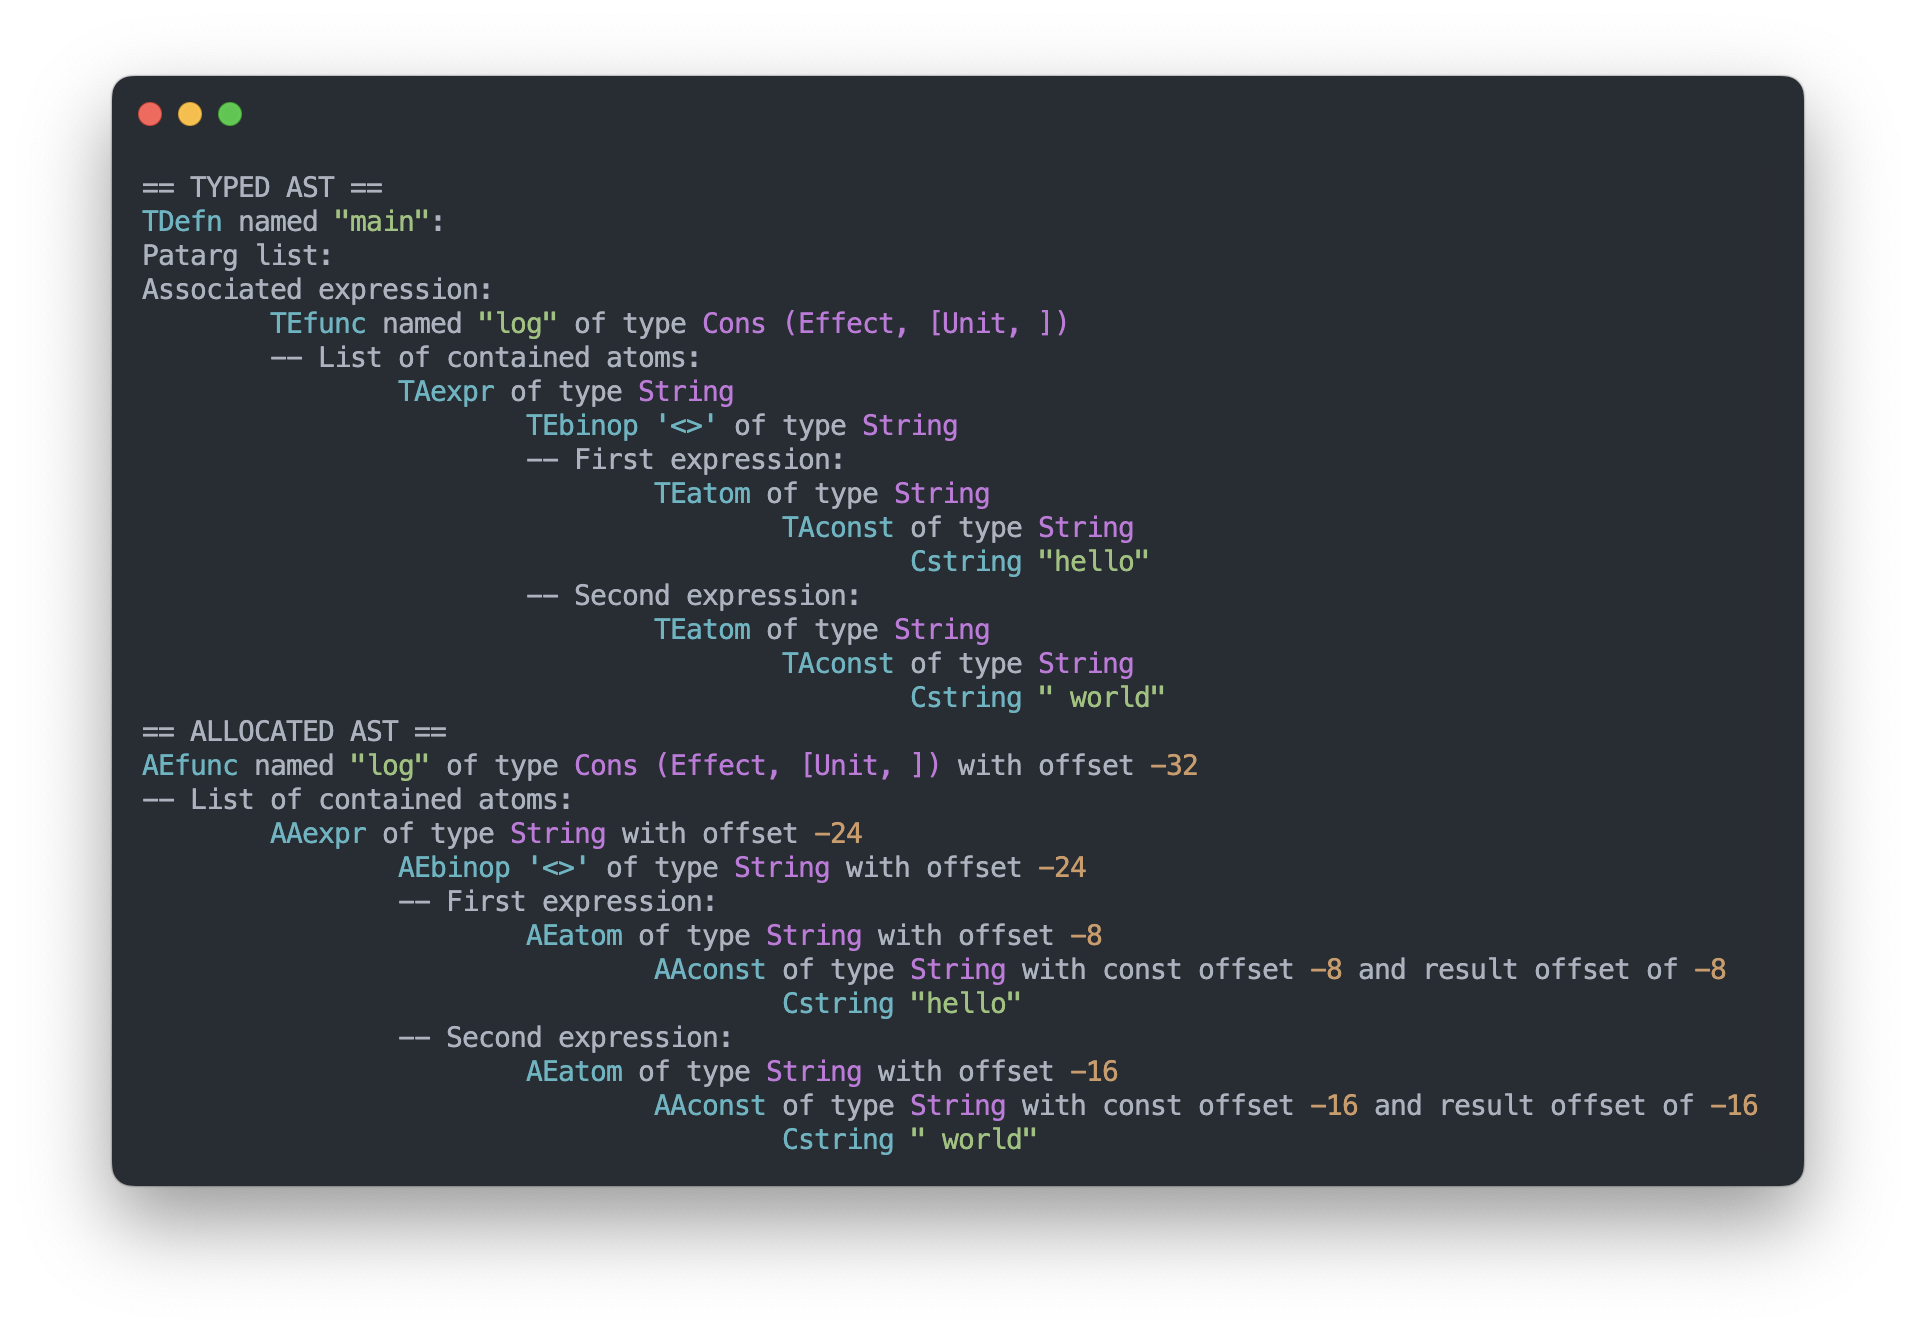
\includegraphics[scale=0.45]{pretty_printer.png}
    \caption{Exemple du \emph{pretty printer} sur \texttt{concat.purs}}
\end{figure}

\section{Limitations connues}
Notre compilateur ne passe pas tous les tests fournis. Ces limitations sont dues aux difficultés rencontrées lors du typage des instances et du \emph{pattern matching}.

Par ailleurs, la gestion de la pile laisse à désirer. Dans certains cas (\texttt{do}, \texttt{if}), il aurait été préférable d'allouer les expressions successivement calculées aux mêmes emplacements sur la pile plutôt que de continuer à allouer en haut de celle-ci. Nous avons néanmoins adopté cette dernière option pour simplifier la gestion des compteurs et ainsi faciliter de déboggage.

\end{document}